\section{Проектирование гибридной интеллектуальной системы}

В соответствии с результатами анализа гибридная интеллектуальная система проектируется как последовательность взаимодействующих компонентов, каждый из которых выполняет ограниченный набор функций. Нейробионический компонент отвечает за получение визуальных наблюдений, тогда как логико-символьный компонент используется для проверки согласованности наблюдений с текущим состоянием шахматной партии и принятия решения о регистрации хода. Дополнительный аналитический компонент обрабатывает уже подтверждённые ходы и не участвует в первичном распознавании изображения.

\subsection{Определение пользователей гибридной интеллектуальной системы}

Основным пользователем системы является игрок или наблюдатель, которому требуется автоматически регистрировать партию, проводимую за физической шахматной доской. Пользователь не обязан вручную вводить ходы, однако должен иметь возможность подтвердить неоднозначное состояние доски и просматривать результаты работы системы.

Дополнительным пользователем является аналитик партии. Его задача заключается в просмотре зарегистрированной партии, отдельных позиций, результатов анализа ходов и сформированных системой сообщений о спорных ситуациях.

Внешними подсистемами являются источник видеоданных и подсистема шахматного анализа. Источник видеоданных предоставляет последовательность кадров, а подсистема шахматного анализа получает уже подтверждённую позицию и выполняет вычислительно более затратный анализ без влияния на основной цикл регистрации.

\begin{table}[htbp]
\centering
\caption{Пользователи и внешние подсистемы}
\begin{tabular}{|>{\raggedright\arraybackslash}p{0.24\textwidth}|>{\raggedright\arraybackslash}p{0.25\textwidth}|>{\raggedright\arraybackslash}p{0.43\textwidth}|}
\hline
\textbf{Категория} & \textbf{Роль} & \textbf{Основные функции} \\
\hline
Игрок или наблюдатель & Основной пользователь & Запуск и завершение регистрации, контроль текущего состояния, подтверждение неоднозначных ситуаций, просмотр текущей позиции и ходов. \\
\hline
Аналитик партии & Пользователь анализа & Просмотр зарегистрированной партии, позиций, оценок ходов и отчёта об игре. \\
\hline
Источник видеоданных & Внешняя подсистема & Передача видеопотока или последовательности изображений шахматной доски. \\
\hline
Подсистема шахматного анализа & Внешняя интеллектуальная подсистема & Оценка подтверждённых позиций и ходов, поиск рекомендованных продолжений и формирование аналитических характеристик партии. \\
\hline

\end{tabular}
\end{table}

\begin{figure}[htbp]
\centering
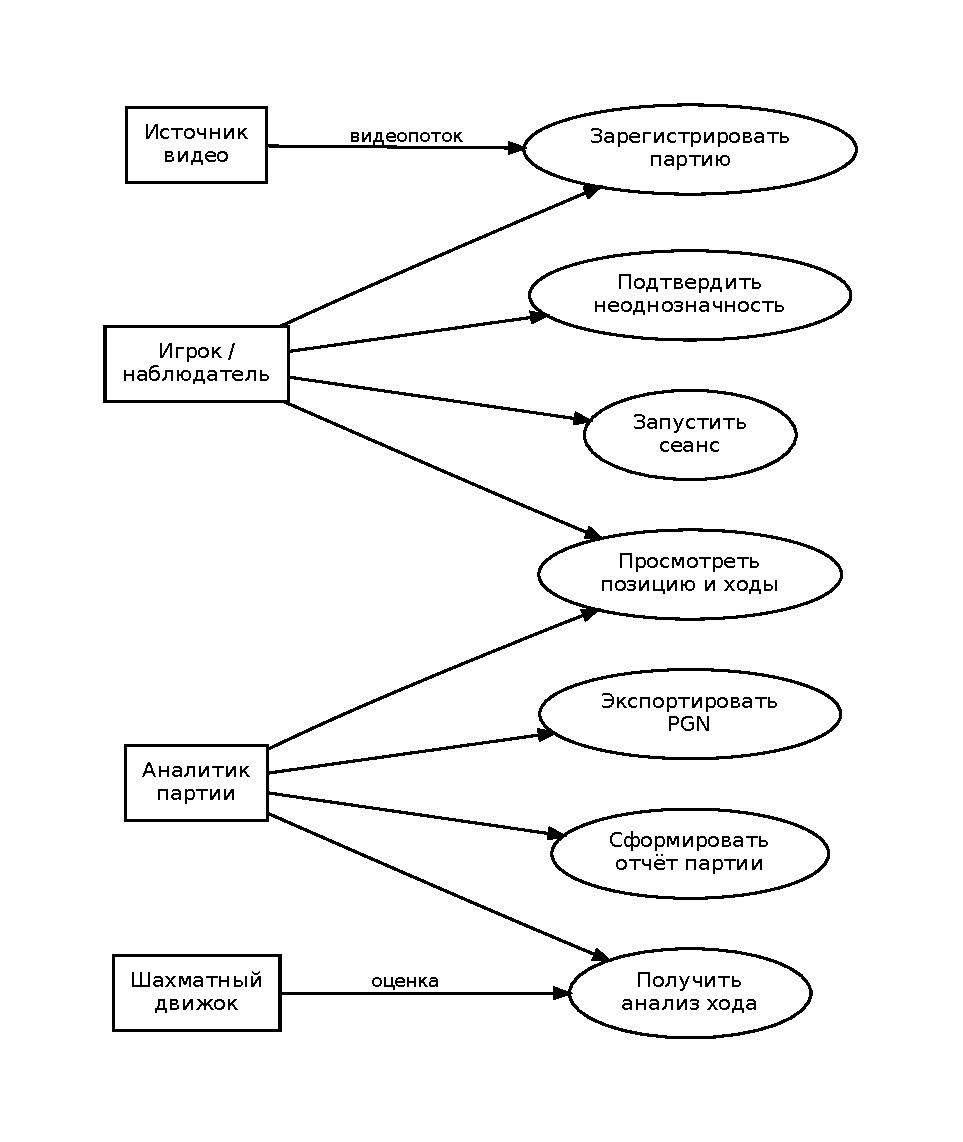
\includegraphics[width=0.88\textwidth]{picture/design_figures/use_case.pdf}
\caption{Диаграмма вариантов использования гибридной интеллектуальной системы}
\label{fig:design-usecase}
\end{figure}

Диаграмма вариантов использования на рисунке~\ref{fig:design-usecase} показывает, что центральным сценарием является регистрация партии. Дополнительные действия пользователя связаны с управлением сеансом, просмотром текущей позиции, разрешением неоднозначностей и получением аналитического результата.

\subsection{Сценарии использования гибридной интеллектуальной системы}

\subsubsection{Сценарий регистрации шахматной партии}

Инициатором сценария является игрок или наблюдатель. Перед началом работы источник видеоданных должен быть доступен, а в поле зрения камеры должна находиться шахматная доска. В ходе инициализации система определяет положение доски и строит её нормализованное представление. После успешной инициализации начинается наблюдение за изменениями положения фигур.

Основной поток имеет следующий вид:

\begin{enumerate}
    \item пользователь запускает сеанс регистрации;
    \item система получает видеоданные и определяет область шахматной доски;
    \item выполняется геометрическая нормализация изображения;
    \item доска разбивается на 64 клетки;
    \item для клеток формируются визуальные наблюдения о наличии фигуры, её цвете и типе;
    \item наблюдения объединяются во временную последовательность и проверяются на устойчивость;
    \item после обнаружения завершившегося движения формируется набор кандидатов хода;
    \item кандидаты проверяются относительно текущей шахматной позиции;
    \item согласованный кандидат фиксируется как новый ход партии;
    \item обновлённое состояние партии сохраняется, а подтверждённый ход передаётся в подсистему анализа.
\end{enumerate}

Граничным случаем является ситуация, при которой часть доски закрыта рукой или фигура находится в движении. В этом случае отдельные наблюдения маркируются как ненадёжные и не должны непосредственно изменять состояние партии. Система продолжает сбор кадров до получения устойчивого наблюдения.

Ошибочным сценарием считается невозможность построить согласованный переход между предыдущей и новой позицией. В этом случае автоматически регистрируется состояние неоднозначности, после чего выполняется повторная обработка ограниченного множества изменившихся клеток. При сохранении неоднозначности пользователь получает запрос на подтверждение.

\subsubsection{Сценарий анализа зарегистрированного хода}

После фиксации хода изменённое состояние передаётся в аналитический компонент. Аналитический компонент работает независимо от первичного распознавания и не должен блокировать продолжение видеорегистрации.

Для подтверждённого хода формируются исходная и конечная позиции, оценка изменения положения и рекомендуемое продолжение. По завершении партии система может сформировать сводный отчёт с ключевыми моментами игры и перечнем ходов, существенно изменивших оценку позиции.

\subsubsection{Сценарий разрешения неоднозначности}

При недостаточной уверенности система не должна принудительно выбирать наиболее вероятный класс. Сначала выполняется повторная обработка следующих кадров, затем рассматриваются альтернативные варианты состояний изменившихся клеток. Если хотя бы один вариант образует допустимый шахматный переход с достаточной визуальной поддержкой, он принимается. В противном случае запрос передаётся пользователю.

\begin{figure}[htbp]
\centering
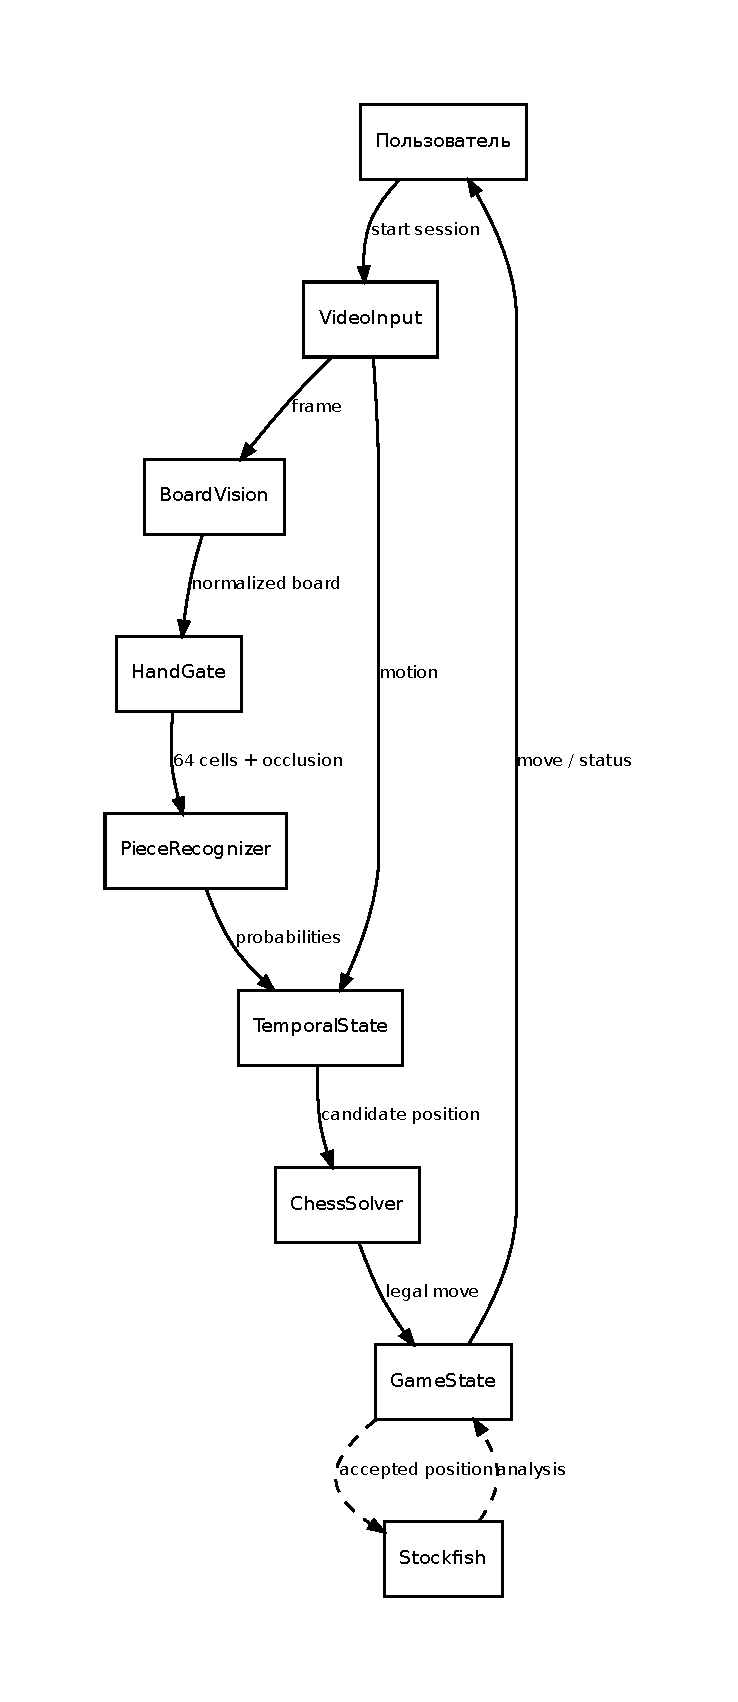
\includegraphics[height=0.75\textheight,width=\textwidth,keepaspectratio]{picture/design_figures/sequence_register.pdf}
\caption{Диаграмма последовательности регистрации одного хода}
\label{fig:design-sequence-register}
\end{figure}

На рисунке~\ref{fig:design-sequence-register} представлено взаимодействие основных компонентов при штатной регистрации хода. Принципиально важным является разделение этапов получения визуального наблюдения и этапа логической проверки: нейробионический компонент предлагает наблюдение, но окончательное изменение состояния партии выполняется после проверки шахматным решателем.

\begin{figure}[htbp]
\centering
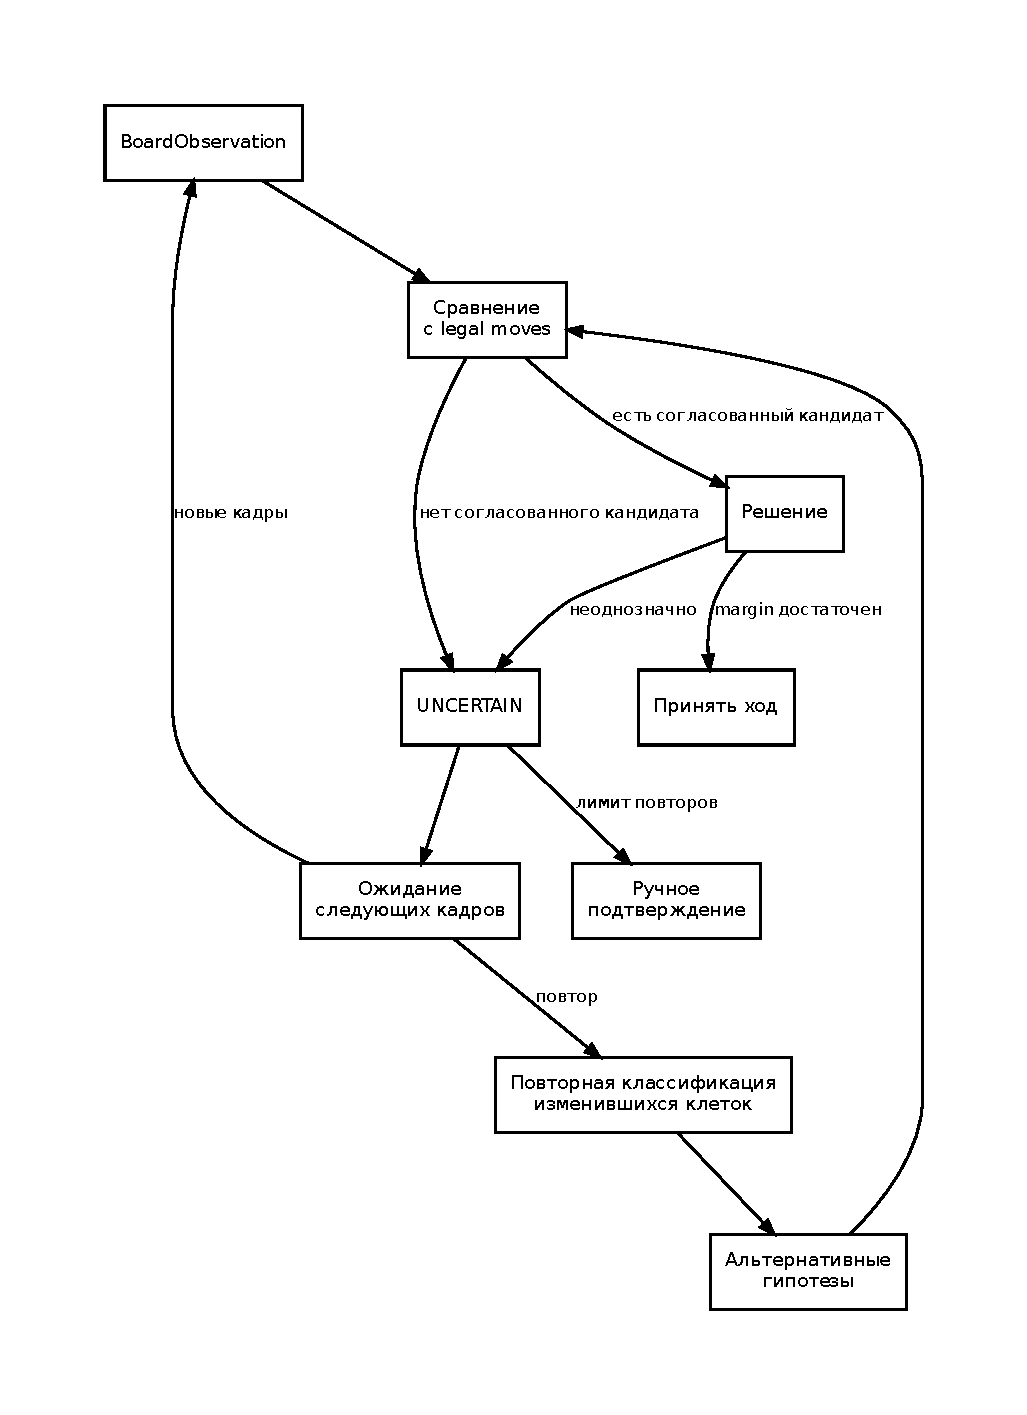
\includegraphics[height=0.75\textheight,width=\textwidth,keepaspectratio]{picture/design_figures/sequence_recovery.pdf}
\caption{Диаграмма последовательности обработки неоднозначного наблюдения}
\label{fig:design-sequence-recovery}
\end{figure}

На рисунке~\ref{fig:design-sequence-recovery} показана ветвь отказоустойчивой обработки. При отсутствии допустимого перехода система не изменяет принятую позицию, а инициирует повторную обработку. Это обеспечивает принцип <<сначала подтвердить состояние, затем изменить его>>.

\subsection{Общая архитектура гибридной интеллектуальной системы}

Архитектура системы разделена на контур визуального восприятия, контур принятия решения и контур последующего анализа. Внутри визуального контура используются средства компьютерного зрения и нейробионический компонент распознавания. Контур принятия решения содержит временную модель состояния, базу знаний предметной области и решатель допустимых шахматных переходов. Аналитический контур запускается после подтверждения хода.

\begin{figure}[htbp]
\centering
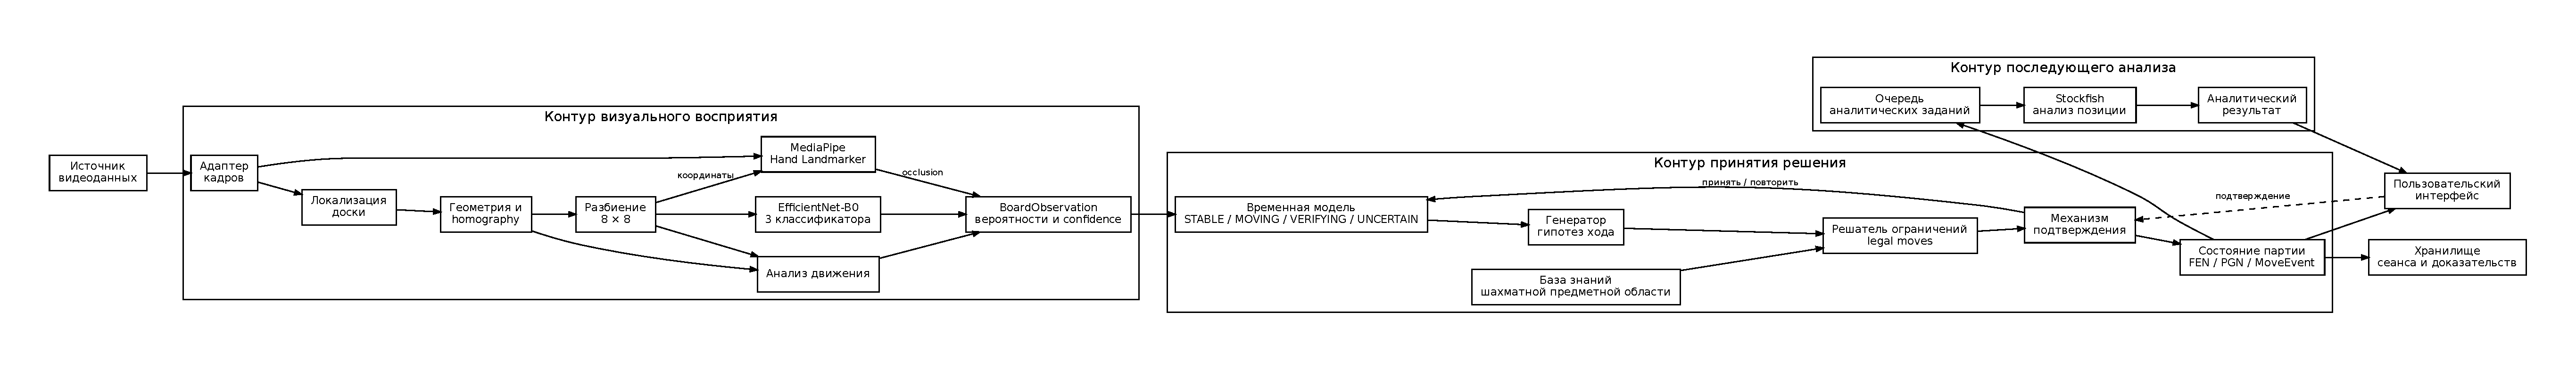
\includegraphics[width=\textwidth]{picture/design_figures/architecture.pdf}
\caption{Общая компонентная архитектура гибридной интеллектуальной системы}
\label{fig:design-architecture}
\end{figure}

Входным элементом является адаптер видеоданных. Для уменьшения вычислительной нагрузки кадры обрабатываются с регулируемой частотой. На этапе инициализации или при потере качества геометрической модели выполняется локализация доски. После получения её границ строится преобразование перспективы, позволяющее привести доску к нормализованному квадратному представлению.

Важным элементом архитектуры является компонент определения перекрытия рукой. В качестве основного средства для этой задачи используется \textbf{MediaPipe Hand Landmarker}. Его роль ограничивается обнаружением положения кисти и её перекрытия с клетками доски. MediaPipe не участвует в поиске самой доски и не используется для распознавания шахматных фигур. Результат работы этого компонента используется как дополнительный признак достоверности: клетки, пересекающиеся с областью руки, временно исключаются из принятия окончательного решения.

Распознавание содержимого клеток выполняется отдельным нейробионическим компонентом. В основной реализации выбран предварительно обученный \textbf{EfficientNet-B0} с тремя классификационными головами: наличие фигуры, цвет и тип фигуры. Обработка 64 клеток выполняется пакетно, что снижает количество вызовов модели. Полученный результат сохраняется в виде распределений вероятностей, а не только в виде одного класса.

Для определения завершения движения используется анализ изменения нормализованных кадров. При обнаружении движения система переходит в состояние ожидания и не фиксирует новые шахматные состояния. После прекращения движения выполняется несколько последовательных наблюдений, на основании которых определяется устойчивое состояние.

Логико-символьный контур обеспечивает предметную валидацию и содержит следующие структурированные элементы:

\begin{itemize}
    \item \textbf{База знаний предметной области}, состоящая из двух взаимосвязанных уровней:
    \begin{itemize}
        \item \textit{декларативный уровень (онтологическая модель):} описывает сущности предметной области (фигуры $\mathcal{P}$, цвета $\mathcal{C}$, поля доски $\mathcal{S}$, топологию смежности и диагоналей), материальные инварианты (единственность королей каждого цвета, инвариант однопольности слонов до превращения, предельное число фигур каждого типа) и допустимые шаблоны перемещений;
        \item \textit{продукционный уровень (правила логического вывода):} формулирует систему продукций вида <<ЕСЛИ условие ТО вывод/действие>> для дедуктивного доопределения типа фигуры при неполных визуальных данных (например, при превращении пешки на 1-й или 8-й горизонтали), отсечения недопустимых ходов под связкой короля и фильтрации оптических артефактов;
    \end{itemize}
    \item \textbf{Решатель шахматных ограничений}, генерирующий строго детерминированное множество легальных ходов $M(B_t)$ для текущего состояния и проверяющий согласованность наблюдаемого перехода;
    \item \textbf{Механизм оценки кандидатов}, сопоставляющий визуальные вероятности с допустимыми ходами;
    \item \textbf{Модуль управления состоянием}, реализующий автомат перехода между фазами стабильности, движения, проверки и устранения неопределенности.
\end{itemize}

На границе между нейробионическим и логико-символьным подходами используется промежуточная структура \texttt{BoardObservation}. Она содержит распределения вероятностей по 64 клеткам, оценки качества геометрии, информацию о движении и маску перекрытых клеток. Благодаря этому логический решатель не зависит от конкретного формата ответа нейронной модели.

\begin{figure}[htbp]
\centering
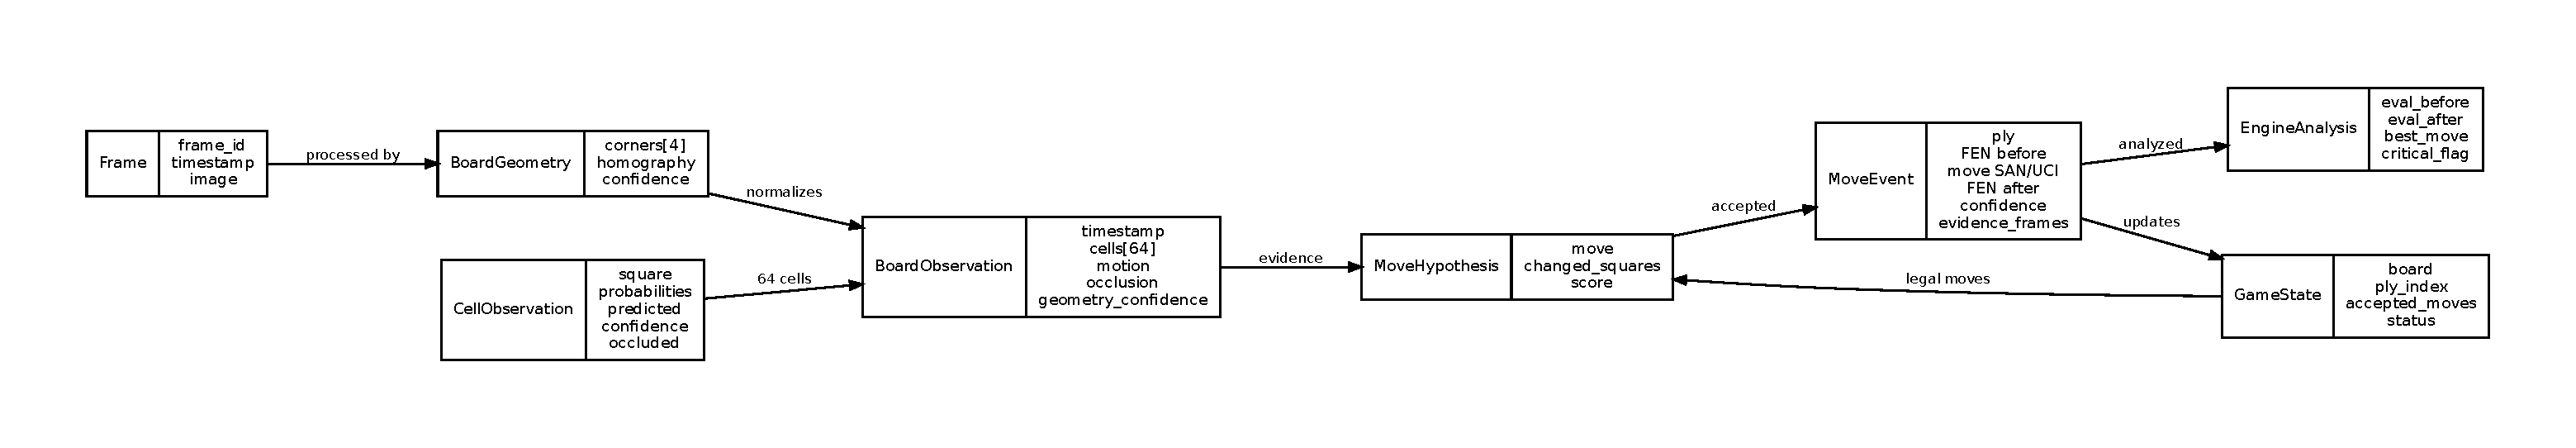
\includegraphics[width=0.94\textwidth]{picture/design_figures/data_model.pdf}
\caption{Основные информационные структуры системы}
\label{fig:design-data-model}
\end{figure}

Система использует два класса состояния данных. Первый представляет текущую принятую шахматную позицию и историю ходов. Второй содержит доказательства принятого решения: номера кадров, изменившиеся клетки, оценки распознавания, состояние геометрии и результаты логической проверки. Это позволяет восстанавливать причину каждого автоматически зарегистрированного хода.

Для устойчивости к потере отдельных компонентов используется принцип независимости контуров. Сбой подсистемы шахматного анализа не должен останавливать регистрацию. Отказ обнаружения руки не должен приводить к немедленной регистрации хода, поскольку дополнительно используются анализ движения и временная стабилизация. Потеря геометрии доски переводит систему в режим ожидания и запрещает изменение шахматного состояния до восстановления геометрии.

\subsection{Проектирование алгоритмов и методов решения задач}

\subsubsection{Алгоритм локализации и нормализации доски}

Для грубой локализации используется одношаговый детектор объектов с одним классом ``board''. В основной реализации применяется лёгкая модель семейства YOLO. Детектор запускается при начале сеанса и периодически повторяется только при ухудшении качества текущей геометрии. Такой режим не требует выполнять обнаружение доски на каждом кадре.

Полученная область уточняется классическими методами компьютерного зрения. Находятся кандидаты на внешние границы доски, после чего проверяются следующие свойства: выпуклость четырёхугольника, положительная площадь, отсутствие самопересечений и возможность однозначно сопоставить его вершины с четырьмя углами нормализованной доски.

После получения четырёх углов вычисляется матрица перспективного преобразования (гомографии). Нормализованный размер доски принят равным $640\times640$ пикселей. 

Важнейшей задачей геометрического этапа является \textbf{определение пространственной ориентации доски} ($a1 \leftrightarrow h8$). Поскольку четырёхугольник доски обладает вращательной симметрией ($90^\circ$ и $180^\circ$), привязка вершин к шахматной системе координат осуществляется по трёхфакторной схеме:
\begin{enumerate}
    \item \textit{правило цветности углов FIDE:} правое нижнее поле относительно любого из игроков всегда является белым (поля $h1$ для стороны белых и $a8$ для стороны чёрных), что исключает ошибочную ориентацию с поворотом на $90^\circ$ или $270^\circ$;
    \item \textit{анализ начального распределения фигурных масс:} при старте партии оценивается занятость противоположных краёв доски. Горизонтали 1--2 и 7--8 содержат фигуры белого и чёрного цвета соответственно, что однозначно разрешает поворот на $180^\circ$;
    \item \textit{параметр конфигурации сеанса:} при нестандартных условиях освещения или старте с произвольной позиции допускается явная фиксация стороны оператора (камера со стороны белых или чёрных).
\end{enumerate}

Кроме того, при нарезке доски на 64 участка учитывается \textbf{эффект перспективного параллакса и трёхмерной высоты фигур}. При углах наклона камеры $\theta < 90^\circ$ (эксплуатационный диапазон $\theta \in [60^\circ, 85^\circ]$) высокие фигуры (короли, ферзи, ладьи) выступают за пределы плоской клетки основания и визуально перекрывают клетки вышестоящих горизонталей. Для компенсации этого эффекта область интереса каждой клетки (Cell ROI) формируется с адаптивным вертикальным расширением на коэффициент $\alpha_{\text{height}} \approx 1{,}25$ вверх вдоль луча наклона перспективы, а классификатор приоритетно взвешивает область основания фигуры, контактирующую с полем доски.

\begin{figure}[htbp]
\centering
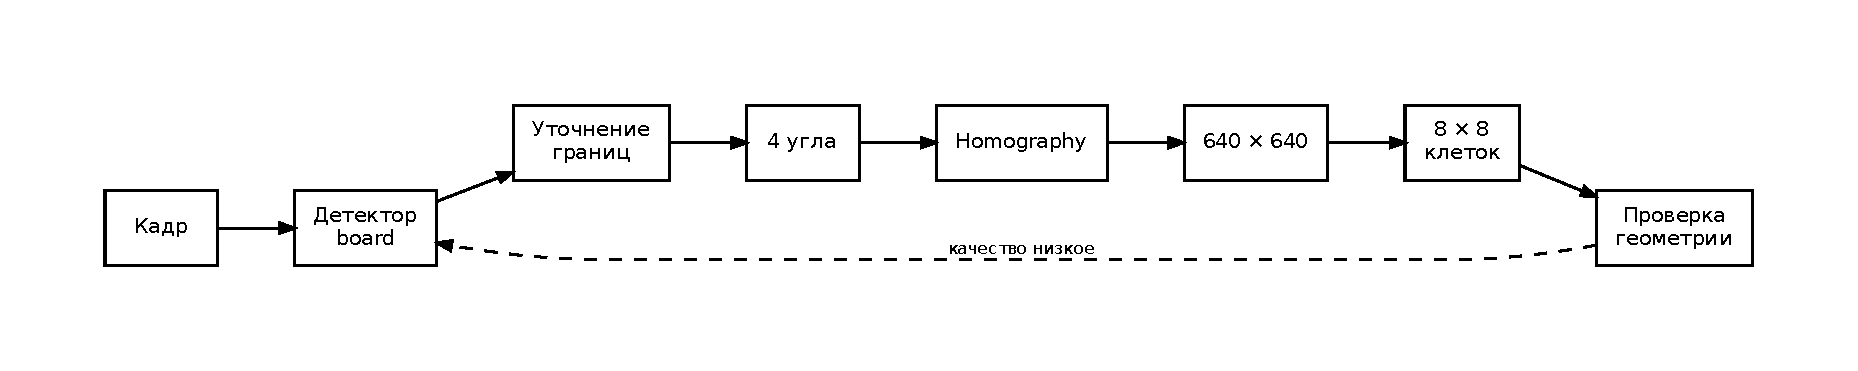
\includegraphics[width=0.92\textwidth]{picture/design_figures/board_pipeline.pdf}
\caption{Последовательность локализации и нормализации шахматной доски}
\label{fig:design-board-pipeline}
\end{figure}

Качество геометрии оценивается по нескольким признакам. Если хотя бы одно из обязательных условий не выполняется, текущая позиция доски не используется для регистрации хода. Это существенно надёжнее попытки продолжать обработку с приблизительными координатами клеток.

\subsubsection{Алгоритм распознавания состояния клетки}

Из каждого нормализованного кадра извлекаются 64 внутренних участка. Обработка выполняется одним пакетным вызовом нейросетевой модели. Основная модель представляет собой предварительно обученный EfficientNet-B0 с дополнительными классификационными головами.

Первая голова определяет состояние \texttt{empty/occupied}. Вторая и третья головы определяют цвет и тип фигуры и активируются для занятых клеток. Итоговое состояние клетки формируется только при согласованности этих признаков.

Пусть $p_o$ обозначает вероятность занятости клетки, $p_c$ --- распределение по цвету, а $p_t$ --- распределение по типу фигуры. Для пустой клетки используется условие
\[
p_o(\text{empty}) \geq \tau_o.
\]
Для занятой клетки дополнительно проверяются
\[
p_o(\text{occupied}) \geq \tau_o,\qquad
\max p_c \geq \tau_c,\qquad
\max p_t \geq \tau_t,
\]
где $\tau_o$, $\tau_c$ и $\tau_t$ являются параметрами конфигурации.

Если хотя бы один из порогов не выполнен, клетка получает состояние \texttt{UNCERTAIN}, а её распределение вероятностей сохраняется для дальнейшего поиска альтернативных вариантов.

\subsubsection{Обнаружение перекрытия руки}

Для этой задачи применяется MediaPipe Hand Landmarker. Компонент обрабатывает исходный или нормализованный кадр и возвращает положение ключевых точек руки. По ограничивающей области обнаруженной руки строится маска перекрытия.

Для каждой клетки вычисляется пересечение с маской. Если площадь пересечения превышает заданный порог, клетка получает признак \texttt{occluded = true}. Такие клетки временно исключаются из принятия окончательного решения.

При физической игре рука оказывает не только прямое экранирующее воздействие, но и \textbf{косвенное оптическое возмущение}:
\begin{itemize}
    \item возникновение резких динамических теней от кисти игрока при направленном комнатном освещении, вызывающих ложные всплески в межкадровой разности;
    \item кратковременное дрожание фигуры при установке на клетку и микроколебания пальцев при отпускании (фаза <<поправляю>>);
    \item перекрытие фигур дальнего плана предплечьем.
\end{itemize}

Таким образом, MediaPipe выступает специализированным вспомогательным сенсором. Отсутствие обнаруженной кисти не гарантирует полного отсутствия оптического шума: для полной фильтрации артефактов вводится межкадровый анализ движения и фаза временной выдержки.

\subsubsection{Временная стабилизация наблюдений}

Независимая обработка каждого кадра приводит к ложным изменениям состояния из-за шумов, теней, бликов и перемещения фигуры между клетками. Поэтому фиксация нового состояния выполняется только после стабилизации.

Состояния автомата показаны на рисунке~\ref{fig:design-state}.

\begin{figure}[htbp]
\centering
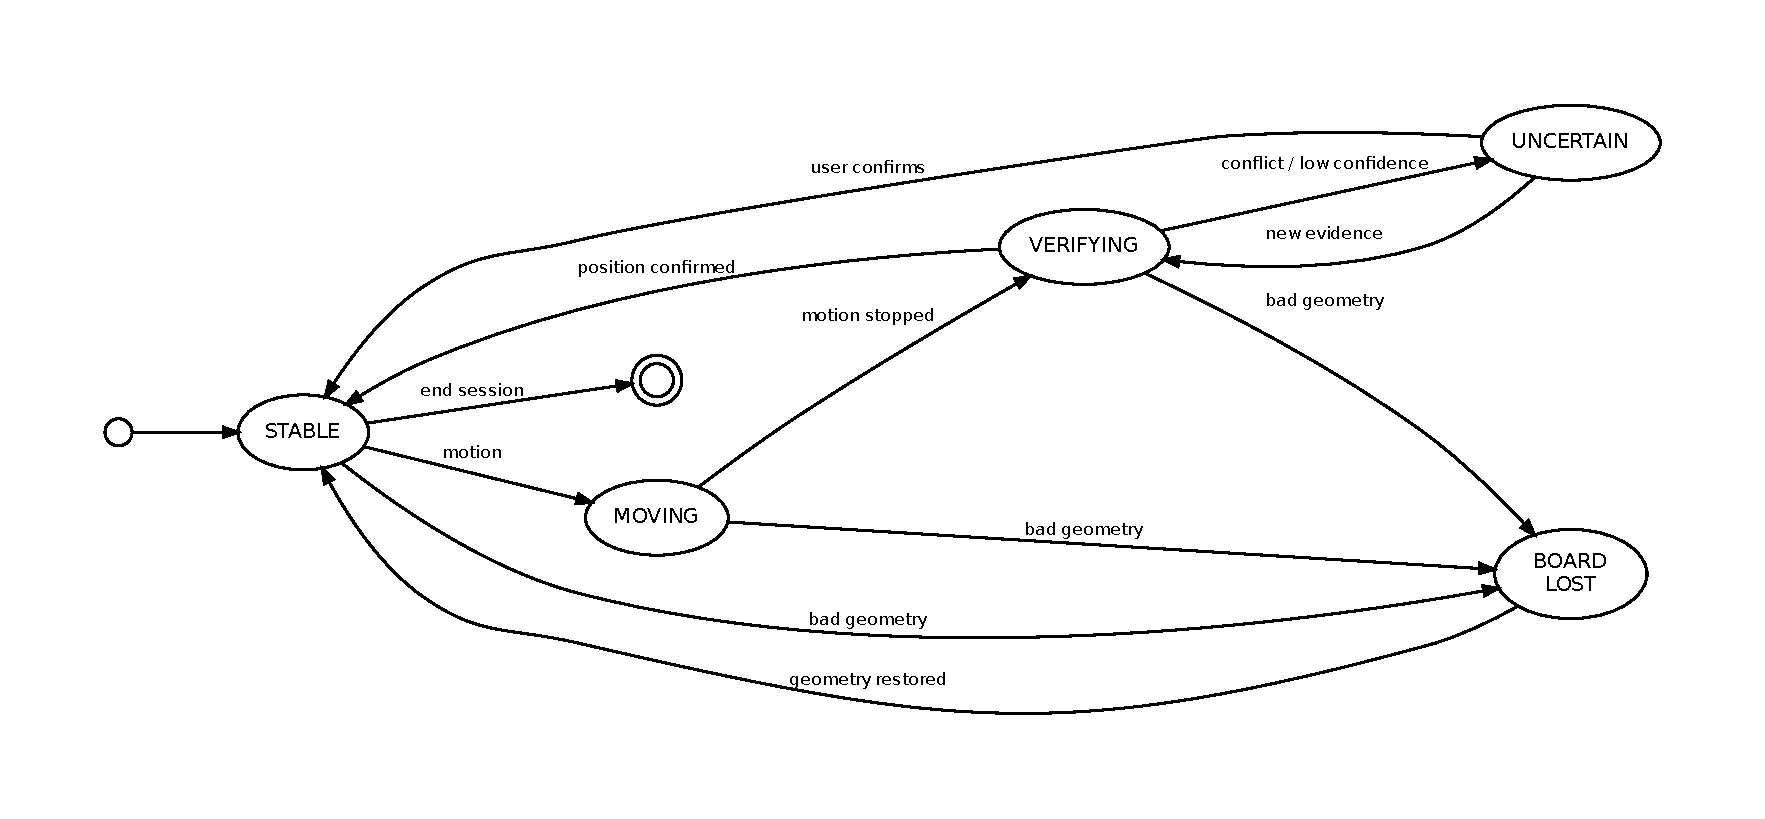
\includegraphics[width=0.92\textwidth]{picture/design_figures/state_machine.pdf}
\caption{Диаграмма состояний процесса регистрации партии}
\label{fig:design-state}
\end{figure}

После обнаружения движения система переходит из состояния \texttt{STABLE} в \texttt{MOVING}. Пока наблюдается движение или перекрытие значимой области, принятие нового состояния строго запрещено. 

После исчезновения движения и выхода кисти из игровой зоны система переходит не сразу к регистрации, а в фазу \textbf{дебаунсинга (временной выдержки)} с интервалом $\Delta t_{\text{settle}} \in [0{,}5; 1{,}0]$~с (15--30 последовательных кадров при 30 кадрах/с). Этот интервал необходим для полного рассеяния динамических теней, затухания механического дрожания фигур и автофокусировки камеры. 

Если в течение интервала $\Delta t_{\text{settle}}$ не зафиксировано новых возмущений, автомат переходит в состояние \texttt{VERIFYING}, где серия последовательных кадров используется для формирования усредненного устойчивого наблюдения $O_{t+1}$. Если же наблюдения противоречат друг другу или содержат высокую долю неопределённых клеток, система переходит в \texttt{UNCERTAIN}. Только после подтверждения непротиворечивого перехода система возвращается в \texttt{STABLE}.

\subsubsection{Формирование кандидатов хода}

Визуальная классификация не определяет ход напрямую. Система сопоставляет текущее устойчивое наблюдение $O_{t+1}$ с принятым состоянием $B_t$, формируя множество изменившихся клеток $\Delta \mathcal{S} = \{s \in \mathcal{S} \mid \text{Diff}(s) > \theta_{\text{diff}}\}$.

Сопоставление наблюдаемых изменений с пространством легальных ходов $M(B_t)$ опирается на \textbf{топологические сигнатуры ходов}:
\begin{itemize}
    \item \textbf{Стандартный ход или простое взятие:} $|\Delta \mathcal{S}| = 2$. Фиксируется освобождение клетки $s_{\text{from}}$ и занятие клетки $s_{\text{to}}$. При взятии на клетке $s_{\text{to}}$ происходит смена цвета или типа фигуры;
    \item \textbf{Рокировка (Castling):} $|\Delta \mathcal{S}| = 4$. Происходит одновременное изменение положений короля и ладьи (для короткой рокировки белых: $e1, g1, h1, f1$; для длинной рокировки: $e1, c1, a1, d1$). Логический контур проверяет взаимную согласованность перемещения обеих фигур как неделимого игрового акта;
    \item \textbf{Взятие на проходе (En Passant):} $|\Delta \mathcal{S}| = 3$. Пешка перемещается на пустую клетку $s_{\text{to}}$, а сбитая пешка противника исчезает с соседней клетки $s_{\text{captured}}$ той же горизонтали;
    \item \textbf{Превращение пешки (Promotion):} $|\Delta \mathcal{S}| = 2$, при этом класс фигуры на целевом поле последней горизонтали (8 для белых, 1 для чёрных) дедуктивно обновляется с пешки на одну из старших фигур ($\text{Q, R, B, N}$).
\end{itemize}

Для каждого кандидата $m \in M(B_t)$, согласующегося с топологической сигнатурой, вычисляется комплексный балл правдоподобия:
\[
S(m) = w_v S_v(m) + w_t S_t(m) + w_g S_g(m) - w_o P_o(m),
\]
где слагаемые формализуются следующим образом:
\begin{itemize}
    \item $S_v(m) = \sum_{s \in \Delta \mathcal{S}} \ln P(c_s^{(m)} \mid O_{t+1}) + \lambda \sum_{s \notin \Delta \mathcal{S}} \ln P(c_s^{(B_t)} \mid O_{t+1})$ --- логарифмическое правдоподобие согласованности вероятностей нейросетевого классификатора с гипотезой $m$;
    \item $S_t(m) \in [0, 1]$ --- показатель стабильности визуального наблюдения на протяжении окна $\Delta t_{\text{settle}}$;
    \item $S_g(m) \in [0, 1]$ --- мера качества перспективной гомографии доски (оценка сохранения параллельности и пропорций);
    \item $P_o(m) = \sum_{s \in \Delta \mathcal{S}} \text{Occlusion}(s)$ --- штрафная функция за частичное перекрытие ключевых полей маской руки;
    \item $w_v, w_t, w_g, w_o$ --- нормированные весовые коэффициенты ($\sum w_i = 1$).
\end{itemize}

Дополнительно проверяется запас уверенности между лучшим $m_1$ и вторым $m_2$ кандидатами:
\[
S(m_1) - S(m_2) \geq \Delta.
\]
Если порог $\Delta$ не достигнут, решение считается спорным, и система переходит в режим добора кадров либо запроса подтверждения.

\begin{figure}[htbp]
\centering
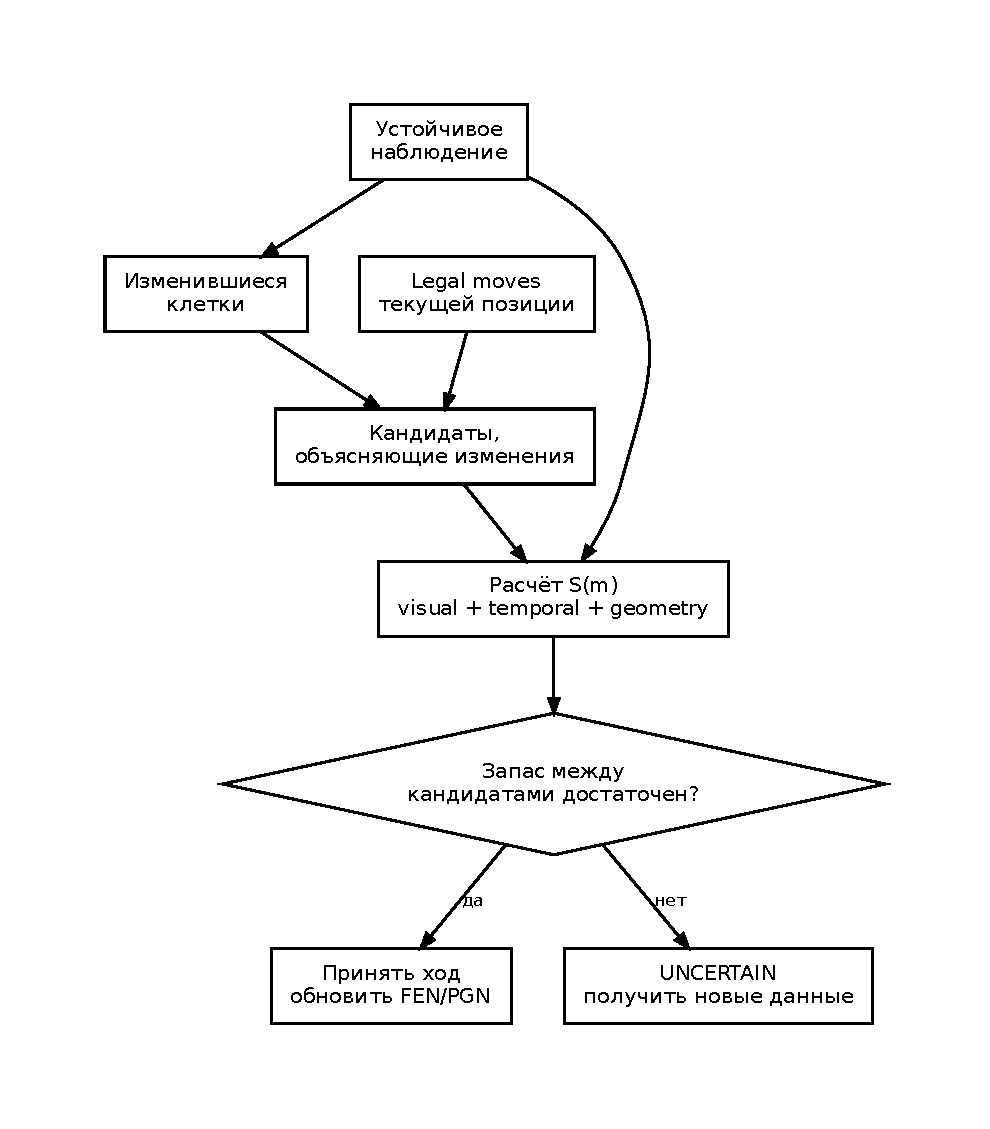
\includegraphics[width=0.94\textwidth]{picture/design_figures/move_decision.pdf}
\caption{Алгоритм выбора и подтверждения хода}
\label{fig:design-move-decision}
\end{figure}

\subsubsection{Проверка шахматных ограничений}

Для поддержания логической модели и валидации ходов используется символьный движок \texttt{python-chess}. Внутреннее состояние формализуется стандартным объектом доски, а после каждого подтверждённого хода строится FEN и PGN-нотация. 

Символьный решатель строго ограничивает поиск гипотез: кандидаты генерируются исключительно из легальных переходов текущей позиции. Это гарантирует невозможность регистрации недопустимых ходов (например, хода связанной фигурой, игнорирования шаха или хода не в свою очередь).

Основной цикл проверки имеет вид:

\begin{verbatim}
previous_position <- accepted game state
observation <- stabilized visual observation
changed <- detect changed squares (topological signatures)
candidates <- legal_moves(previous_position)
candidates <- filter_by_changed_squares(candidates, changed)
score each candidate using S(m)
if best candidate score >= threshold and margin >= Delta:
    apply candidate to accepted game state
    save MoveEvent(ply, FEN, move, evidence)
    dispatch to async analysis queue
else:
    enter UNCERTAIN and request more evidence / prompt user
\end{verbatim}

Такое разделение ответственности лежит в основе гибридной парадигмы: нейросетевая модель оперирует неполными и зашумленными пиксельными данными, а логико-символьный контур отсекает физически и семантически невозможные интерпретации.

\subsubsection{Механизм восстановления после ошибок}

Отказоустойчивость реализуется каскадом действий с возрастающей стоимостью вычислений.

При первой ошибке система ожидает несколько следующих кадров. Если этого недостаточно, выполняется повторная классификация только изменившихся клеток. Затем рассматриваются альтернативные классы клеток с наибольшими вероятностями. После этого повторяется поиск допустимого шахматного перехода.

Если ни один вариант не приводит к согласованному состоянию, текущая принятая позиция сохраняется без изменений. Пользователю отображается конкретная область неоднозначности, а не сообщение об общей ошибке. После подтверждения система может продолжить регистрацию с последней подтверждённой позиции.

Для исключения потери партии после перезапуска каждый подтверждённый ход должен быть атомарно сохранён вместе с FEN до хода и FEN после хода. Повторная запись того же хода должна быть идемпотентной и не должна увеличивать номер полухода.

\subsubsection{Постобработка подтверждённого хода}

После фиксации хода его результаты передаются в движок шахматного анализа \textbf{Stockfish}. Анализ не участвует в распознавании изображения и выполняется асинхронно.

Для каждого хода сохраняются:

\begin{itemize}
    \item оценка позиции до хода;
    \item оценка позиции после хода;
    \item рекомендуемое продолжение;
    \item изменение оценки;
    \item признаки потенциально критического хода.
\end{itemize}

На основании этих данных формируется дополнительный интеллектуальный слой системы. Он может отображать текущее состояние партии, предупреждать о существенном ухудшении оценки, выделять критические моменты и после завершения партии формировать краткий отчёт.

При этом результат движка не изменяет зарегистрированный ход. Это принципиально: если игрок сделал допустимый, но не лучший ход, система должна зарегистрировать фактически выполненное действие и отдельно сообщить его оценку.

\subsubsection{Порядок обработки одного цикла}

Полный цикл работы системы представляет собой следующий последовательный процесс:

\begin{enumerate}
    \item получение очередного кадра;
    \item проверка наличия и качества модели доски;
    \item преобразование перспективы;
    \item получение маски перекрытий;
    \item выделение 64 клеток;
    \item пакетная классификация клеток при необходимости;
    \item формирование \texttt{BoardObservation};
    \item оценка движения и обновление автомата состояний;
    \item при переходе в \texttt{VERIFYING} --- построение кандидатов новой позиции;
    \item проверка кандидатов относительно текущей позиции;
    \item принятие хода или запуск процедуры восстановления;
    \item сохранение \texttt{MoveEvent};
    \item передача подтверждённого состояния в аналитический компонент.
\end{enumerate}

\begin{figure}[htbp]
\centering
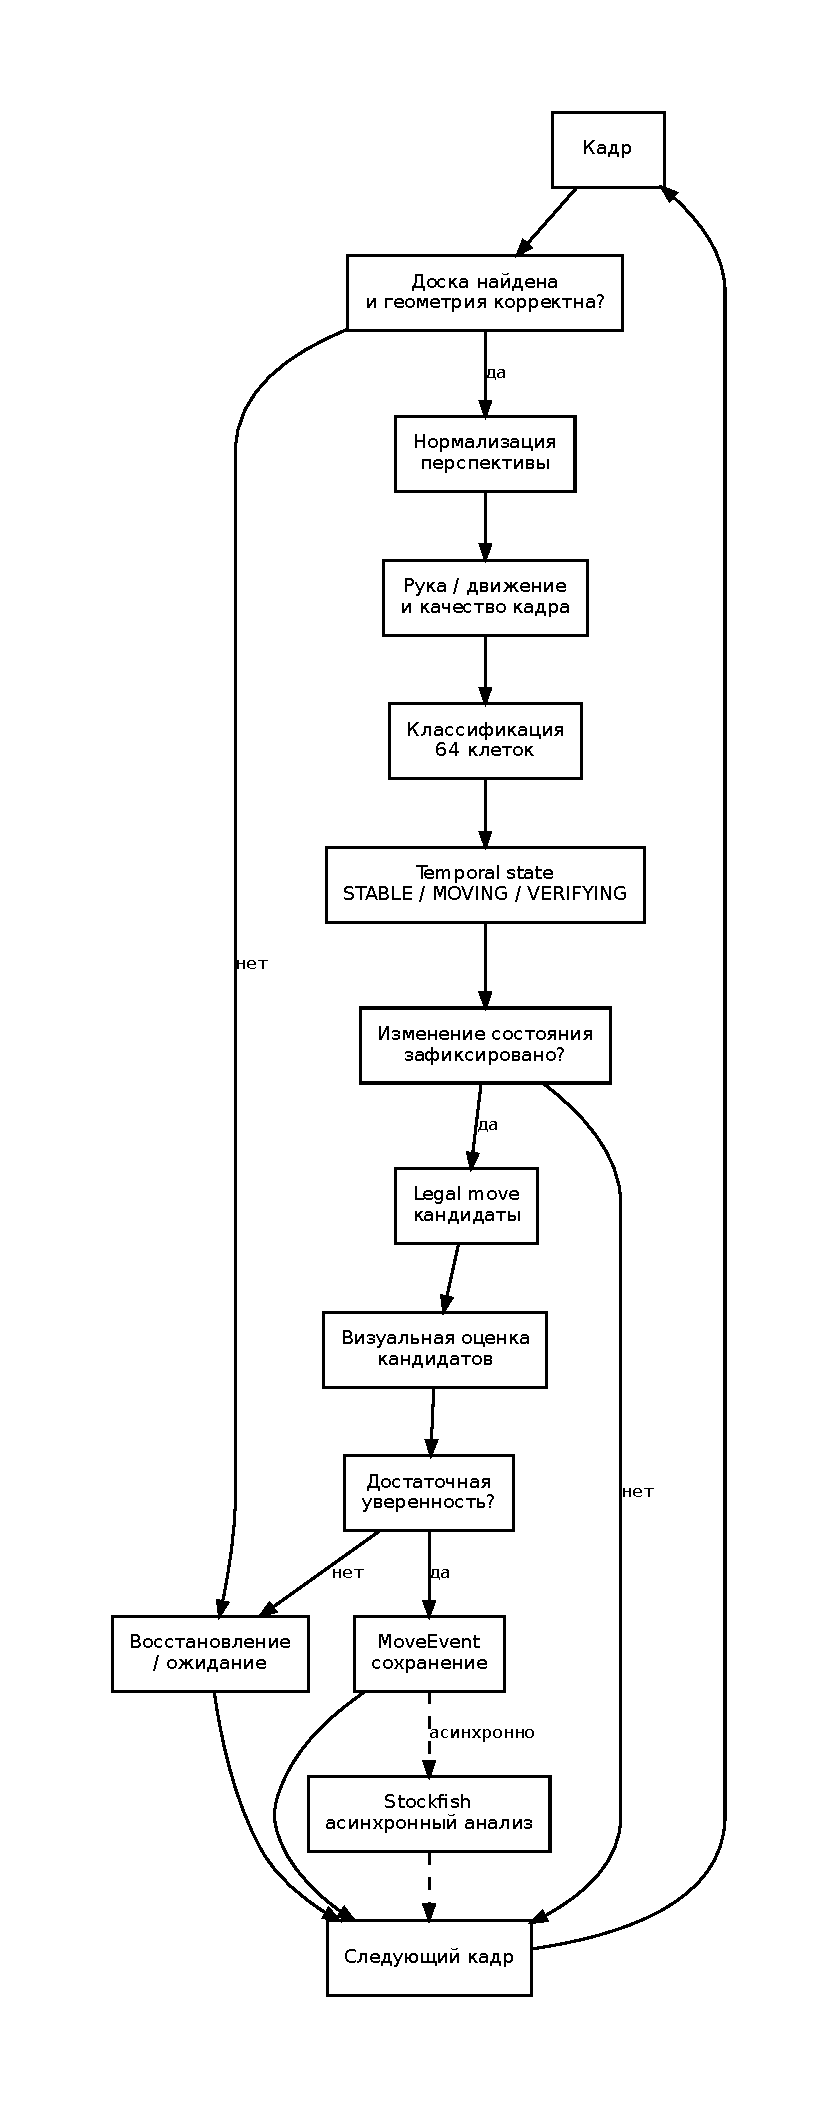
\includegraphics[height=0.75\textheight,width=\textwidth,keepaspectratio]{picture/design_figures/full_cycle.pdf}
\caption{Общий алгоритм работы гибридной интеллектуальной системы}
\label{fig:design-full-cycle}
\end{figure}

\subsubsection{Стратегия вычислительной нагрузки}

Чтобы обеспечить возможность обучения и эксплуатации на ограниченных вычислительных ресурсах, наиболее затратные операции не выполняются на каждом кадре.

Локализация доски выполняется при начале сеанса и повторяется только при ухудшении оценки геометрии. Обработка руки выполняется на отобранных кадрах текущего цикла. Классификация клеток выполняется пакетно и особенно часто запускается после обнаружения движения, когда изменение состояния действительно возможно. В устойчивом состоянии достаточно выполнять редкие контрольные наблюдения.

Таким образом, вычислительная нагрузка распределяется следующим образом:

\begin{table}[htbp]
\centering
\caption{Периодичность выполнения основных операций}
\begin{tabular}{|>{\raggedright\arraybackslash}p{0.32\textwidth}|>{\raggedright\arraybackslash}p{0.26\textwidth}|>{\raggedright\arraybackslash}p{0.34\textwidth}|}
\hline
\textbf{Компонент} & \textbf{Типичный режим} & \textbf{Причина} \\
\hline
Локализация доски & При запуске и при потере геометрии & Неизменность положения доски между соседними кадрами. \\
\hline
Геометрическое преобразование & Для каждого анализируемого кадра & Нормализованное пространство является общей системой координат. \\
\hline
Обнаружение руки & На анализируемом кадре & Необходимо учитывать текущее перекрытие доски. \\
\hline
Классификация 64 клеток & При обнаружении изменения и на контрольных кадрах & Нет необходимости выполнять тяжёлую классификацию при полном отсутствии изменений. \\
\hline
Проверка legal moves & Только после формирования кандидата & Проверяется только небольшой набор возможных переходов. \\
\hline
Stockfish & После подтверждения хода, асинхронно & Анализ не должен блокировать регистрацию следующего действия. \\
\hline
\end{tabular}
\end{table}

\subsubsection{Форматы обмена данными между компонентами}

Для обеспечения независимости компонентов вводится несколько логических структур данных.

\begin{table}[htbp]
\centering
\caption{Основные структуры данных}
\begin{tabular}{|>{\raggedright\arraybackslash}p{0.28\textwidth}|>{\raggedright\arraybackslash}p{0.64\textwidth}|}
\hline
\textbf{Структура} & \textbf{Содержимое} \\
\hline
\texttt{Frame} & Идентификатор кадра, временная метка, изображение. \\
\hline
\texttt{BoardGeometry} & Четыре угла доски, матрица перспективного преобразования, оценка качества геометрии. \\
\hline
\texttt{CellObservation} & Координата клетки, распределения вероятностей, итоговый класс, уверенность и признак перекрытия. \\
\hline
\texttt{BoardObservation} & 64 наблюдения клеток, состояние движения, маска перекрытия, оценка качества доски и временная метка. \\
\hline
\texttt{MoveHypothesis} & Кандидат хода, изменившиеся клетки, визуальная оценка и суммарный балл. \\
\hline
\texttt{MoveEvent} & Номер полухода, FEN до и после, SAN/UCI, временная отметка, уверенность, ссылки на доказательные кадры и результаты анализа. \\
\hline
\end{tabular}
\end{table}

\subsubsection{Обработка типовых отказов}

Проектируемая система должна сохранять последнюю подтверждённую позицию при любом сбое, который не позволяет доказать следующий ход. Для разных типов отказов используются разные стратегии.

\begin{table}[htbp]
\centering
\caption{Обработка отказов и неоднозначных состояний}
\begin{tabular}{|>{\raggedright\arraybackslash}p{0.32\textwidth}|>{\raggedright\arraybackslash}p{0.60\textwidth}|}
\hline
\textbf{Ситуация} & \textbf{Действие системы} \\
\hline
Доска не найдена & Сохранить последнее состояние, продолжить поиск доски, не регистрировать ход. \\
\hline
Плохая геометрия & Не обновлять позицию, повторить оценку границ и перспективы. \\
\hline
Рука закрывает клетки & Пометить клетки как ненадёжные, дождаться освобождения области. \\
\hline
Низкая уверенность классификатора & Сохранить распределение вероятностей, получить дополнительные кадры и альтернативные гипотезы. \\
\hline
Ни один кандидат не является legal move & Запустить процедуру восстановления; при неуспехе запросить подтверждение. \\
\hline
Недоступен шахматный движок & Продолжить регистрацию партии без аналитического слоя, пометив результат анализа как недоступный. \\
\hline
Разрыв видеопотока & Перевести сеанс в состояние ожидания и продолжить с последней сохранённой позиции после восстановления потока. \\
\hline
Сбой приложения & Восстановить последнюю позицию из журнала подтверждённых ходов и не создавать дублирующий ход. \\
\hline
\end{tabular}
\end{table}

\subsubsection{Оценка вычислительной сложности}

Для одной итерации основного контура число клеток фиксировано и равно 64, поэтому сложность обработки клеток определяется вычислительной стоимостью одного пакетного запуска нейросетевой модели. Геометрическое преобразование имеет линейную зависимость от числа пикселей нормализованного изображения. Генерация legal moves выполняется относительно текущей позиции и не зависит от количества кадров до хода.

Для поиска кандидатов существенным является не количество всех возможных конфигураций доски, а размер множества legal moves текущей позиции. Ограничение кандидатов по изменившимся клеткам дополнительно сокращает число сравнений визуальных гипотез.

Memory footprint определяется в основном размером видеобуфера, параметрами нейросетевой модели и хранилищем доказательных кадров. Для предотвращения неограниченного роста диска доказательные кадры рекомендуется хранить ограниченно: полный набор кадров вокруг неоднозначного хода и сокращённый набор для уверенных ходов.

\subsubsection{Интеграция аналитического слоя}

После принятия хода логико-символьный решатель обновляет состояние партии и формирует новый FEN. Аналитический слой получает этот FEN и номер хода через очередь задач. Результаты анализа прикрепляются к соответствующему \texttt{MoveEvent} по уникальному идентификатору события.

Разделение регистрации и анализа делает систему устойчивой к различной скорости компонентов. Если аналитический слой временно отстаёт, очередь растёт, но видеорегистрация продолжает работать. При восстановлении аналитическая очередь обрабатывается последовательно. Повторный анализ одного события исключается идентификатором хода.

\subsubsection{Диаграмма состояний системы}

На рисунке~\ref{fig:design-state} показан автомат регистрации. Отдельно от него в реализации поддерживается состояние аналитического задания: \texttt{QUEUED}, \texttt{RUNNING}, \texttt{COMPLETED}, \texttt{FAILED}. Это состояние не влияет на шахматную позицию и может существовать независимо от состояния видеорегистрации.

Таким образом, проектируемая система является гибридной не только по составу технологий, но и по способу принятия решений. Визуальный компонент формирует вероятностное наблюдение, временной компонент отбрасывает нестабильные состояния, логико-символьный компонент ограничивает множество допустимых интерпретаций, а аналитический компонент выполняет последующую оценку уже подтверждённого действия.

\subsection{Выводы}

В результате проектирования определены пользователи и основные сценарии взаимодействия с системой, сформирована компонентная архитектура и разделены зоны ответственности нейробионического и логико-символьного подходов. Основным входом системы является видеопоток, из которого формируется нормализованное представление шахматной доски и вероятностное описание 64 клеток.

Ключевым механизмом надёжности является отказ от непосредственного изменения шахматной позиции по результату одного кадра. Регистрация хода выполняется только после калибровки ориентации ($a1 \leftrightarrow h8$), компенсации перспективного параллакса 3D-высоты фигур, временного дебаунсинга оптических теней, формирования кандидатов по топологическим сигнатурам ходов и проверки их на допустимость относительно текущей позиции. 

Для обработки перекрытий введён отдельный компонент обнаружения руки на основе MediaPipe Hand Landmarker, а для распознавания клеток выбран пакетный нейробионический классификатор на основе EfficientNet-B0. Шахматные ограничения и состояние партии обрабатываются символьным решателем на базе онтологии игры и продукционных правил, а углубленный анализ подтверждённых действий выполняется асинхронным движком Stockfish.

Спроектированная структура данных обеспечивает передачу вероятностных наблюдений между компонентами, сохранение доказательств принятия решения и восстановление состояния после сбоев. Это позволяет рассматривать систему как последовательность независимых модулей с контролируемыми точками интеграции и с явным разделением регистрации фактического хода и последующего анализа его качества.
